\documentclass{standalone}
\usepackage{tikz}
\begin{document}
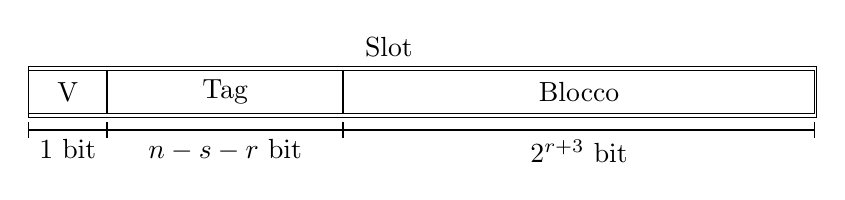
\begin{tikzpicture}
    \draw
    (0,0)node[rectangle, draw, minimum height=0.65cm, minimum width=10cm](b){}
    (b.north)node[above left]{Slot}
    (b.west)node[rectangle,draw,minimum height=0.55cm, minimum width=0.99cm,anchor=west, inner sep=0](v){V}
    (v.east)node[rectangle, draw, minimum height=0.55cm, minimum width=2.98cm, anchor=west, inner sep=0](t){Tag}
    (t.east)node[rectangle, draw, minimum height=0.55cm, minimum width=5.98cm, anchor=west, inner sep=0](b){Blocco}
    (v.south west)++(0,-0.2)coordinate(a1)
    (v.south east)++(0,-0.2)coordinate(a2)
    (t.south east)++(0,-0.2)coordinate(a3)
    (b.south east)++(0,-0.2)coordinate(a4)
    ;
    \draw[|-|](a1)--(a2)node[midway, below]{1 bit};
    \draw[|-|](a2)--(a3)node[midway, below]{$n-s-r$ bit};
    \draw[|-|](a3)--(a4)node[midway, below]{$2^{r+3}$ bit};
\end{tikzpicture}
\end{document}